\documentclass{beamer}
\usepackage[utf8]{inputenc}
\usepackage{amsmath}
\usepackage{wasysym}
\usepackage{svg}
\usepackage{biblatex}
\usepackage{pgfplots}

\bibliography{ref.bib}

\usetheme{Madrid}
\usecolortheme{default}

\title[CSC 592 Project]
{Tuning and Attacking Secure Learned Bloom Filters}

\author
{Calvin Higgins}

\institute[]
{
  Department of Computer Science and Statistics\\
  University of Rhode Island
}

\AtBeginSection[]
{
  \begin{frame}
    \frametitle{Table of Contents}
    \tableofcontents[currentsection]
  \end{frame}
}

\begin{document}

% ------------------------------------------------------------
% Slide
% ------------------------------------------------------------

\frame{\titlepage}

% ------------------------------------------------------------
% Slide
% ------------------------------------------------------------

\begin{frame}
\frametitle{Approximate Membership Query (AMQ) Filters}

\begin{center}
    \includesvg[scale=0.6]{csc592_amq_def.drawio.svg}

    \vspace{1em}
    
    \textbf{Idea:} Check if $x \in S$ with false positive rate $\epsilon$. 
\end{center}

\end{frame}   


% ------------------------------------------------------------
% Slide
% ------------------------------------------------------------

\begin{frame}
\frametitle{Approximate Membership Query (AMQ) Filters}

\begin{center}
    \includesvg[scale=0.6]{csc592_amq_db.drawio.svg}

    \vspace{1em}
    
    \textbf{Motivation:} Cheaply filter database queries to reduce load. 
\end{center}

\end{frame}   

% ------------------------------------------------------------
% Slide
% ------------------------------------------------------------

\begin{frame}
\frametitle{Bloom Filters (BFs) \cite{bloom_1970}}

\begin{center}
    \includesvg[scale=0.5]{csc592_bloom_def.drawio.svg}

    \vspace{1em}

    \textbf{Idea:} Output $x \in S$ iff $x$ maps to all ones.
\end{center}

\end{frame}

% ------------------------------------------------------------
% Slide
% ------------------------------------------------------------

\begin{frame}
\frametitle{Bloom Filters (BFs) \cite{bloom_1970}}

\begin{center}
    \includesvg[scale=0.5]{csc592_bloom_def.drawio.svg}

    \vspace{1em}

    \textbf{Parameters:} The number of hash functions and bits.
\end{center}

\end{frame}

% ------------------------------------------------------------
% Slide
% ------------------------------------------------------------

\begin{frame}
\frametitle{Learned Bloom Filters (LBFs) \cite{kraska_beutel_chi_dean_polyzotis_2018}}


\begin{center}
    \includesvg[scale=0.6]{csc592_lbf_def.drawio.svg}

    \vspace{1em}

    \textbf{Idea:} Try machine learning model and then eliminate false negatives.  
\end{center}

\end{frame}

% ------------------------------------------------------------
% Slide
% ------------------------------------------------------------

\begin{frame}
\frametitle{Learned Bloom Filters (LBFs) \cite{kraska_beutel_chi_dean_polyzotis_2018}}


\begin{center}
    \includesvg[scale=0.6]{csc592_lbf_def.drawio.svg}

    \vspace{1em}

    \textbf{Parameters:} The threshold and Bloom filter false positive rate.
\end{center}

\end{frame}

% ------------------------------------------------------------
% Slide
% ------------------------------------------------------------

\begin{frame}
\frametitle{Threat Model \cite{bishop_tirmazi_2025} \cite{naor_eylon_2019}}

\begin{block}{Adversarial Objective}
    Create \textbf{new} false positives to reduce database performance.
\end{block}

\vspace{1em}

\begin{block}{Adversarial Capabilities}
    The adversary has
    \begin{enumerate}
        \item Polynomial time
        \item Query access to the AMQ filter
        \item White-box access to the AMQ filter
        \item Total control over the set $S$
    \end{enumerate}
\end{block}

\end{frame}


% ------------------------------------------------------------
% Slide
% ------------------------------------------------------------

\begin{frame}
\frametitle{Secure Bloom Filters (SBFs) \cite{naor_eylon_2019}}

\begin{center}
    \includesvg[scale=0.5]{csc592_sbloom_def.drawio.svg}

    \vspace{1em}

    \textbf{Idea:} Replace hash functions with cryptographic hash functions.
\end{center}

\end{frame}

% ------------------------------------------------------------
% Slide
% ------------------------------------------------------------

\begin{frame}
\frametitle{Secure Learned Bloom Filters (SLBFs) \cite{bishop_tirmazi_2025}}

\begin{center}
    \includesvg[scale=0.5]{csc592_slbf_def.drawio.svg}

    \vspace{1em}

    \textbf{Idea:} Double-check machine learning model with secure Bloom filters.
\end{center}

\end{frame}

% ------------------------------------------------------------
% Slide
% ------------------------------------------------------------

\begin{frame}
\frametitle{Secure Learned Bloom Filters (SLBFs) \cite{bishop_tirmazi_2025}}

\begin{center}
    \includesvg[scale=0.5]{csc592_slbf_def.drawio.svg}

    \vspace{1em}

    \textbf{Parameters:} The threshold and secure Bloom filter false positive rates.
\end{center}

\end{frame}

% ------------------------------------------------------------
% Slide
% ------------------------------------------------------------

\begin{frame}
\frametitle{Tuning Secure Learned Bloom Filters (SLBFs)}

\begin{block}{False Positive Rate \cite{bishop_tirmazi_2025}}
    SBLFs have an expected false positive rate of
    \begin{align*}
        \epsilon = \text{M}_\text{FPR} \text{TP}_\text{FPR} + \text{M}_\text{TNR} \text{FN}_\text{FPR}
    \end{align*}
    where $\text{M}$ is the machine learning model, $\text{TP}$ is the true positive filter and $\text{FN}$ is the false negative filter.
\end{block}

\begin{block}{Memory Footprint}
    SLBFs require
    \begin{align*}
        m = -\frac{n}{\ln(2)^2} \left( \text{M}_\text{TPR} \ln(\text{TP}_\text{FPR}) + \text{M}_\text{FNR} \ln(\text{FN}_\text{FPR}) \right) + \text{M}_m + 2 \lambda
    \end{align*}
    bits of memory.
\end{block}

\end{frame}

\begin{frame}
\frametitle{Tuning Secure Learned Bloom Filters (SLBFs)}

\begin{block}{Optimal Secure Bloom Filter False Positive Rates}
    The optimal true positive and false negative filter false positive rates are
    \begin{align*}
        \text{TP}_\text{FPR}^* = \epsilon \frac{\text{M}_\text{TPR}}{\text{M}_\text{FPR}} && \text{FN}_\text{FPR}^* = \epsilon \frac{\text{M}_\text{FNR}}{\text{M}_\text{TNR}}
    \end{align*}
    where $\text{M}$ is the machine learning model, $\text{TP}$ is the true positive filter and $\text{FN}$ is the false negative filter.
\end{block}

\begin{block}{Proof Sketch}
    Express $\text{FN}_\text{FPR}$ in terms of $\text{TP}_\text{FPR}$. Set $\frac{\partial m}{\partial \text{TP}_\text{FPR}} = 0$ and solve for $\text{TP}_\text{FPR}^*$. Substitute to find $\text{FN}_\text{FPR}^*$.
\end{block}

\end{frame}

% ------------------------------------------------------------
% Slide
% ------------------------------------------------------------

\begin{frame}
\frametitle{Tuning Secure Learned Bloom Filters (SLBFs)}

\begin{block}{Optimal Threshold}
    The optimal threshold $\tau^*$ minimizes
    \begin{align*}
        C(\tau) = -\text{M}_\text{TPR} \ln \left( \frac{\text{M}_\text{TPR}}{\text{M}_\text{FPR}} \right) 
 - \text{M}_\text{FNR} \ln \left( \frac{\text{M}_\text{FNR}}{\text{M}_\text{TNR}}\right)
    \end{align*}
    subject to
    \begin{align*}
        \max\left\{\epsilon\frac{\text{M}_\text{TPR}}{\text{M}_\text{FPR}}, \epsilon \frac{\text{M}_\text{FNR}}{\text{M}_\text{TNR}} \right\} \leq \epsilon_\text{max}
    \end{align*}
    and can be found in $\Theta(n \lg n)$ time with dynamic programming!
\end{block}

\end{frame}

% ------------------------------------------------------------
% Slide
% ------------------------------------------------------------

\begin{frame}
\frametitle{Tuning Secure Learned Bloom Filters (SLBFs)}

\begin{center}
    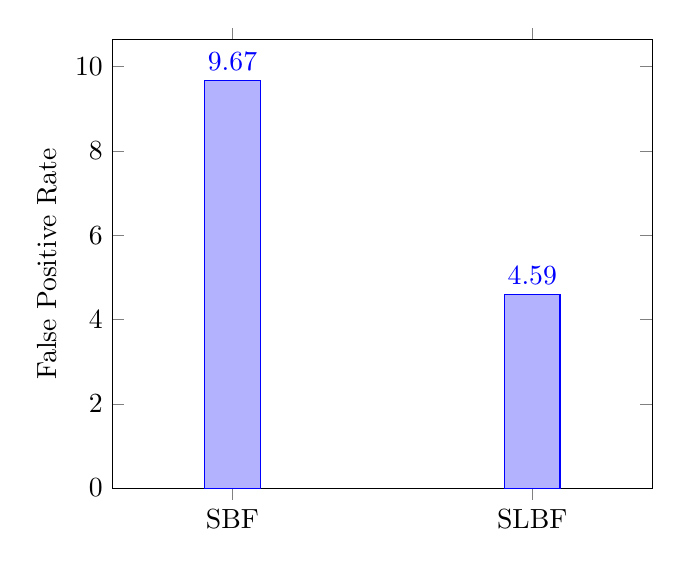
\begin{tikzpicture}
        \begin{axis}[
            ybar,
            symbolic x coords={SBF, SLBF},
            xtick=data,
            ylabel={False Positive Rate},
            ymin=0,
            bar width=20pt,
            nodes near coords,
            enlarge x limits=0.4
        ]
            \addplot coordinates {(SBF, 9.67) (SLBF, 4.59)};
        \end{axis}
    \end{tikzpicture}

    \textcolor{red}{\textbf{SLBFs outperform SBFs under a fixed memory budget!}}
\end{center}

\end{frame}

% ------------------------------------------------------------
% Slide
% ------------------------------------------------------------

\begin{frame}
\frametitle{Attacking Secure Learned Bloom Filters (SLBFs)}

\textbf{Experimental Setup:}
\begin{enumerate}
    \item Truncate/pad $\sim600$K benign/malicious URLs to 128 bytes.
    \item Train a shallow Transformer encoder for URL classification.
    \item Compute optimal SLBF parameter values.
    \item Construct a SLBF ($\epsilon=0.05$, $\epsilon_\text{max} = 0.2$) from the set of malicious URLs.
\end{enumerate}

\end{frame}

% ------------------------------------------------------------
% Slide
% ------------------------------------------------------------

\begin{frame}
\frametitle{Attacking Secure Learned Bloom Filters (SLBFs)}

\textbf{Adaptive Black Box Attack:}
\begin{enumerate}
    \item Create a synthetic SLBF
    \begin{enumerate}
        \item Generate a random set of URLs.
        \item Label the URLs with the SLBF.
        \item Train a deep Transformer encoder on the labeled URLs.
    \end{enumerate}
    \item Create adversarial examples
    \begin{enumerate}
        \item Generate a new random set of URLs.
        \item Embed the URLs with the embedding layer.
        \item Optimize the URL embeddings with Adam to have positive class label.
        \item Unembed the URL embeddings with maximum cosine similarity.
        \item Remove any previously queried URLs with an AMQ filter.
        \item Return the optimized URLs.
    \end{enumerate}
\end{enumerate}

\end{frame}

% ------------------------------------------------------------
% Slide
% ------------------------------------------------------------

\begin{frame}
\frametitle{Attacking Secure Learned Bloom Filters (SLBFs)}

\begin{center}
    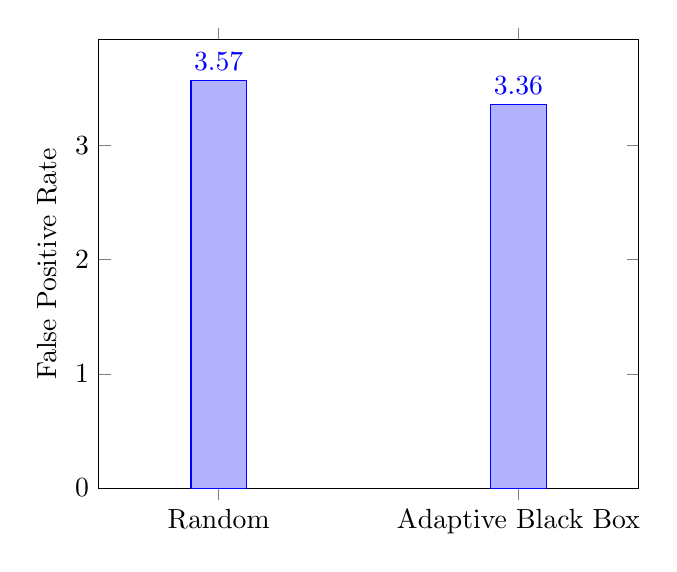
\begin{tikzpicture}
        \begin{axis}[
            ybar,
            symbolic x coords={Random, Adaptive Black Box},
            xtick=data,
            ylabel={False Positive Rate},
            ymin=0,
            bar width=20pt,
            nodes near coords,
            enlarge x limits=0.4
        ]
            \addplot coordinates {(Random, 3.57) (Adaptive Black Box, 3.36)};
        \end{axis}
    \end{tikzpicture}

    \textcolor{blue}{\textbf{No significant difference! ($p = 0.1532, \chi^2 = 266$)}}
\end{center}

\end{frame}

% ------------------------------------------------------------
% Slide
% ------------------------------------------------------------

\begin{frame}
\frametitle{Attacking Secure Learned Bloom Filters (SLBFs)}

\textbf{Targeted Random Attack:}
\begin{enumerate}
    \item Generate a random set of URLs.
    \item Label the random URLs with the learned model.
    \item Split the URLs into two sets by label.
    \item If the true positive filter has higher false positive rate, take the positive URL set, otherwise take the negative URL set.
    \item Remove any previously queried URLs with an AMQ filter.
    \item Return the optimized URLs.
\end{enumerate}

\end{frame}

% ------------------------------------------------------------
% Slide
% ------------------------------------------------------------

\begin{frame}
\frametitle{Attacking Secure Learned Bloom Filters (SLBFs)}

\begin{center}
    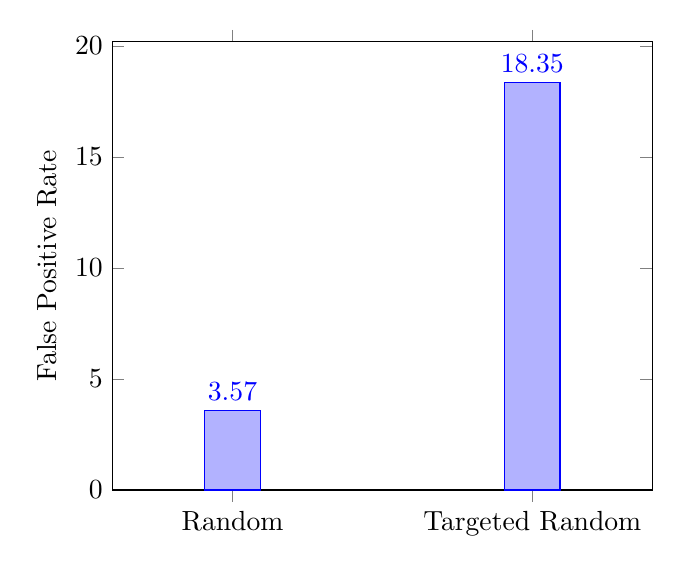
\begin{tikzpicture}
        \begin{axis}[
            ybar,
            symbolic x coords={Random, Targeted Random},
            xtick=data,
            ylabel={False Positive Rate},
            ymin=0,
            bar width=20pt,
            nodes near coords,
            enlarge x limits=0.4
        ]
            \addplot coordinates {(Random, 3.57) (Targeted Random, 18.35)};
        \end{axis}
    \end{tikzpicture}

    \textcolor{blue}{\textbf{Significant but the defense succeeded ($\epsilon_\text{max} = 0.2$)!}}
\end{center}

\end{frame}

% ------------------------------------------------------------
% Slide
% ------------------------------------------------------------

\begin{frame}
\frametitle{Summary of Contributions}

\textbf{Contributions:}
\begin{enumerate}
    \item Implemented Secure Bloom filters
    \item Implemented Secure Learned Bloom filters
    \item Derived optimal parameters for Secure Learned Bloom filters
    \begin{enumerate}
        \item Closed-form solutions for $\text{FN}_\text{FPR}$ and $\text{TP}_\text{FPR}$
        \item Efficient dynamic programming algorithm for $\tau$
    \end{enumerate}
    \item Evaluated the robustness of Secure Learned Bloom filters against
    \begin{enumerate}
        \item Adaptive black box attack
        \item Targeted randomized attack
    \end{enumerate}
\end{enumerate}

\end{frame}

% ------------------------------------------------------------
% Slide
% ------------------------------------------------------------

\begin{frame}
\frametitle{References}

\printbibliography

\end{frame}

\end{document}